\section{Implicit derivering}
Att derivera en given funktion $f(x)$ är lätt med hjälå av regler som till exempel produktregeln och kedjeregeln.
Ibland vill man dock beräkna derivator för kurvor som \underline{inte} är funktionsgrafer,
till exempel\\
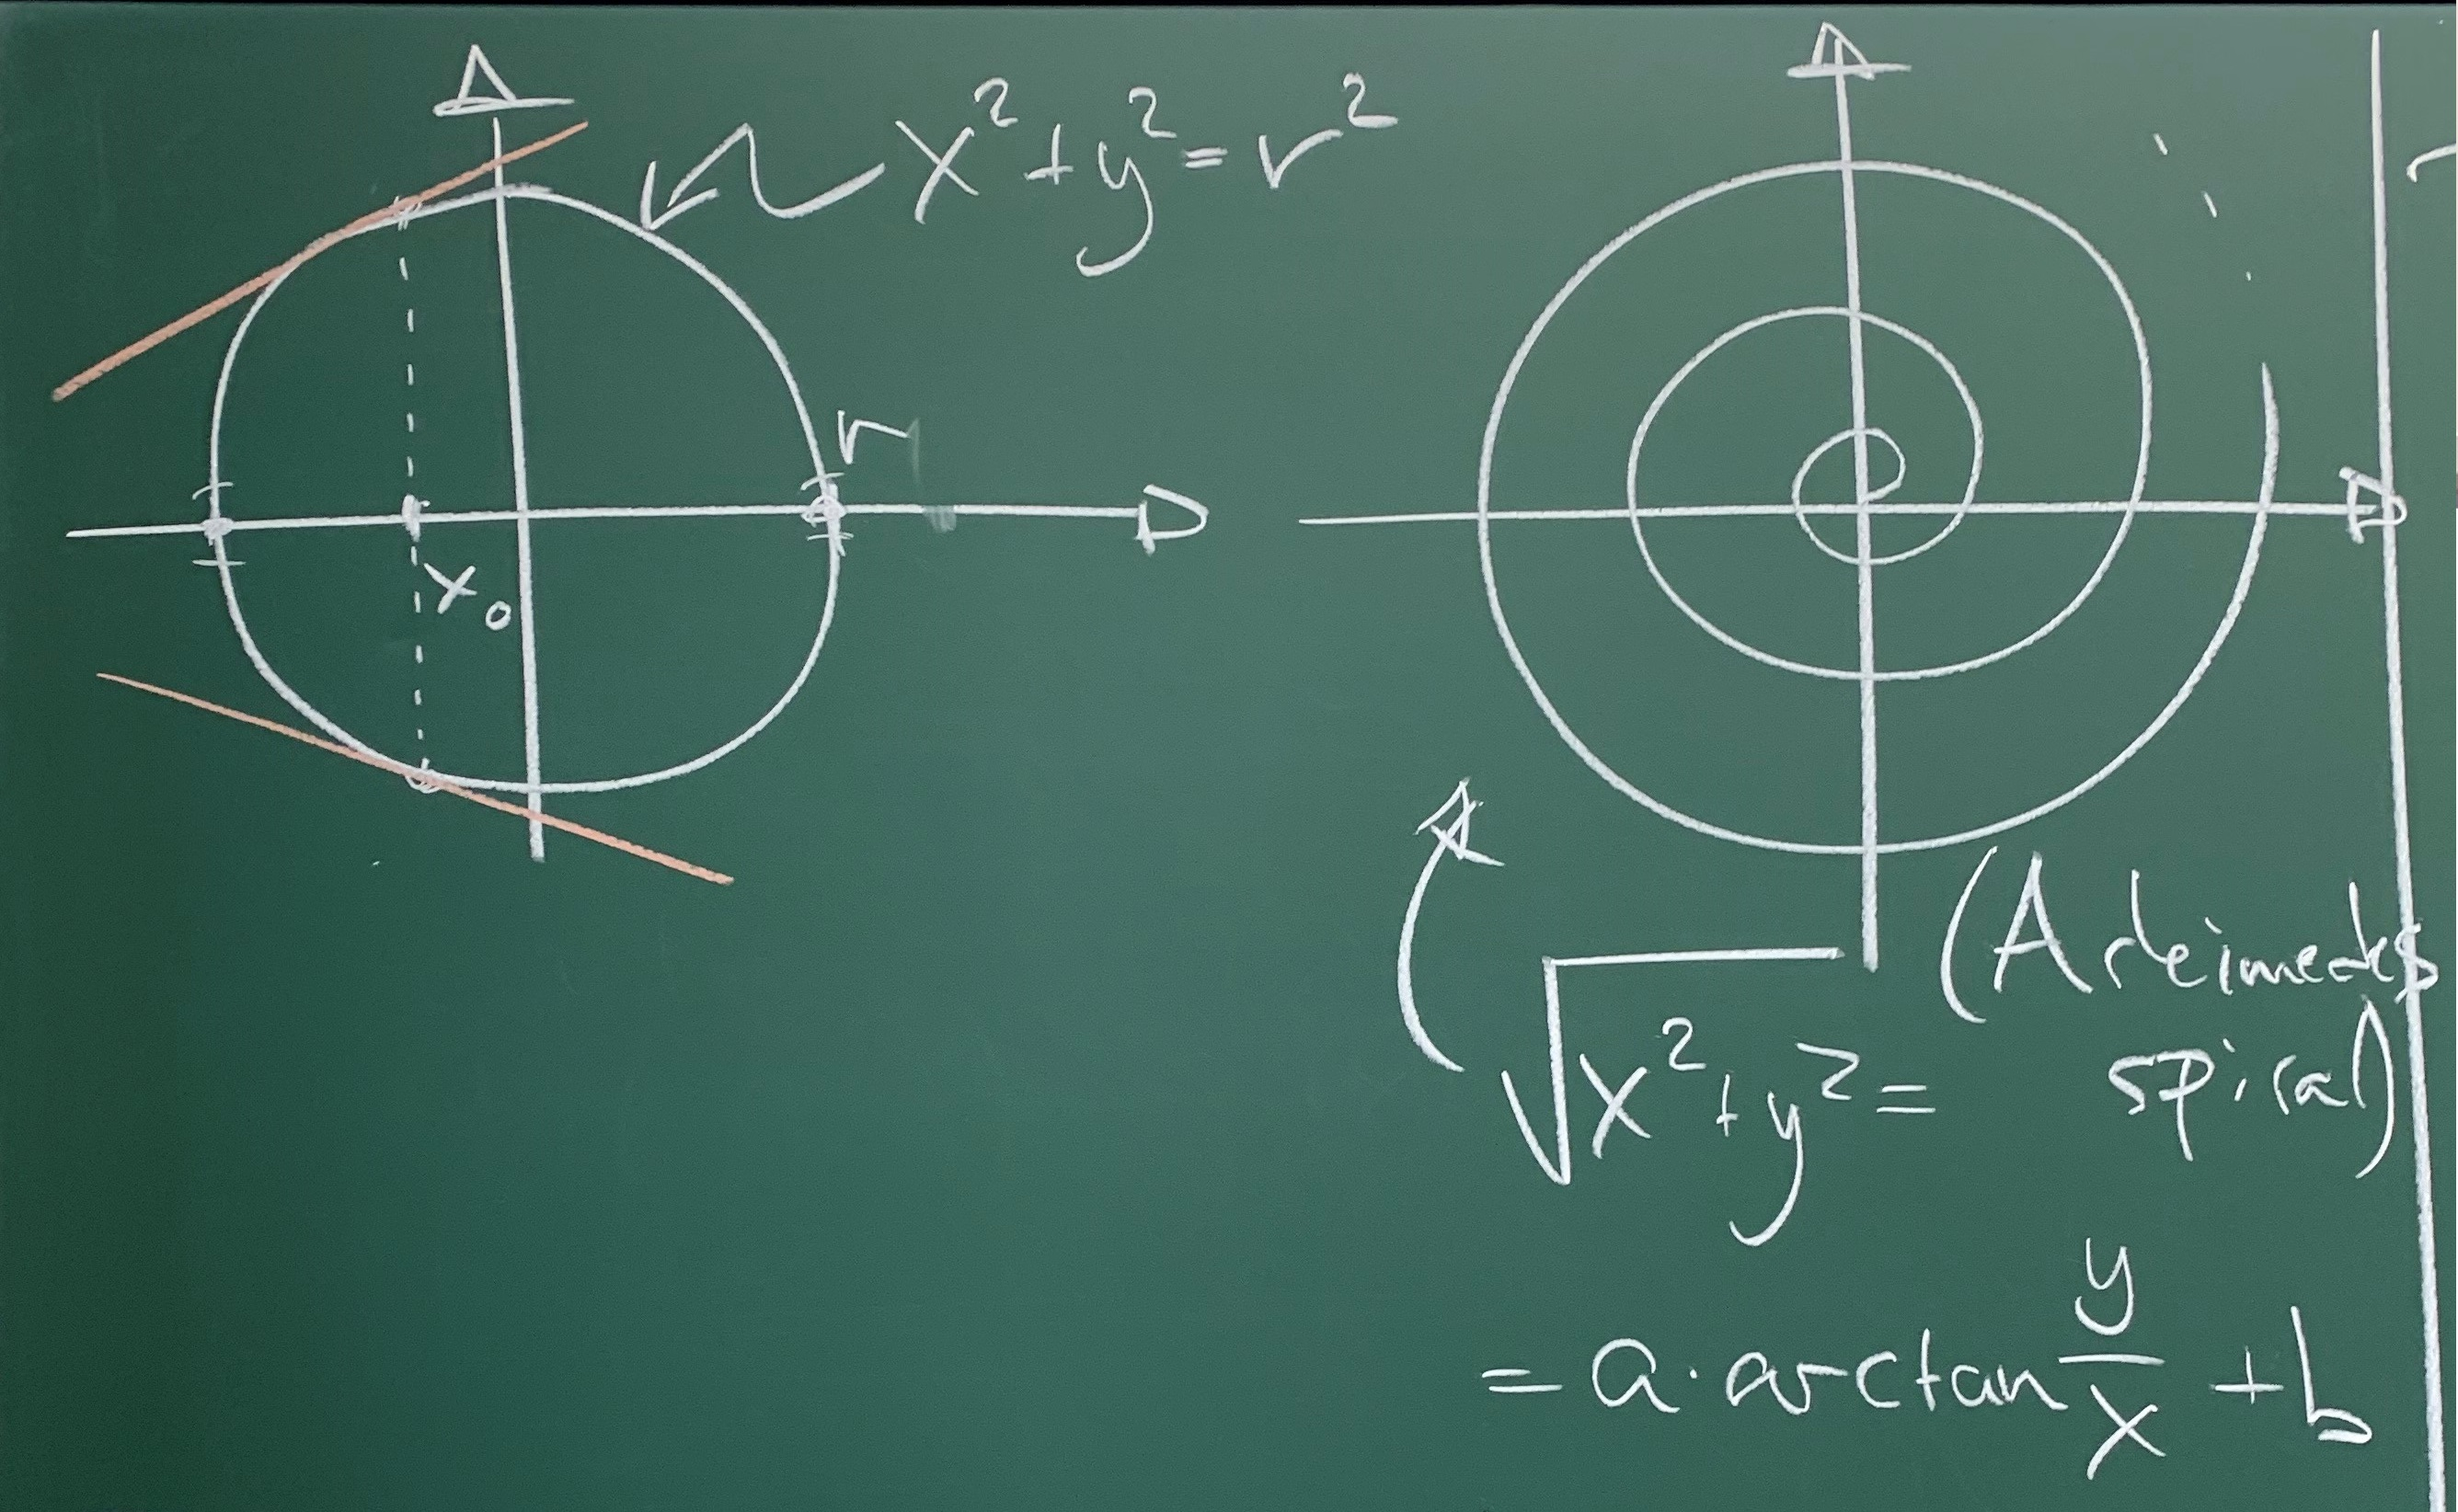
\includegraphics[scale=0.1]{lessons/lesson08/imgs/img01.jpg}\\
Denna typ av kurvor kan inte skrivas på formen $y=f(x)$,
men däremot som $F(x,y)=0$.

\paragraph{Ex} Archimedes spiral kan skrivas $F(x,y)=\sqrt{x^2+y^"}-a\cdot \arctan{\frac{y}{x}}-b$\\
\\
Hur beräknar man kurvan $F(x,y)=0$ i punkten $x=x_0$?
Notera att det mycket väl kan finnas \underline{flera} derivator tillhörande en given punkt $x=x_0$.
Man kan använda kedjeregeln för att beräkna $F^\prime(x,y)$.

\paragraph{Ex (2.9.5)} Givet kurvan $x^2y^3=2x-y$, bestäm $y^\prime$ uttryckt i termer av $x$ och $y$.
\subparagraph{Lösning}
\begin{equation*}
    x^2y^3=2x-y\Leftrightarrow F(x,y)=x^2y^3-2x+y=0
\end{equation*}
\begin{equation*}
    F^\prime(x,y)=\frac{d}{dx}[F(x,y)]=\frac{d}{dx}[x^2y^3-2x+y]=\frac{d}{dx}(x^2y^3)-\frac{d}{dx}(2x)+\frac{d}{dx}(y)=
\end{equation*}
\begin{equation*}
    \{\frac{d}{dx}(2x)=2,\frac{d}{dx}(y)=\frac{dy}{dx}=y^\prime\}=\frac{d}{dx}(x^2x^3)-2+y^\prime=\{\text{produktregeln}\}=
\end{equation*}
\begin{equation*}
    2x\cdot y^3+x^2\cdot\frac{d}{dx}(y^3)-2+y^\prime=\{\text{kedjeregeln}\}=2x\cdot y^3+x^2\cdot 3\cdot y^2\cdot y^\prime-2+y^\prime
\end{equation*}
För kurvan gäller att:
\begin{equation*}
    F(x,y)=0\Rightarrow F^\prime(x,y)=0\Rightarrow 2xy^3+3x^2y^2y^\prime-2+y^\prime=0\Leftrightarrow y^\prime=\frac{2-2xy^3}{1+3x^2y^2}\text{ }\Box
\end{equation*}
\\
Vid implicit derivering måste man vara noga med att ha koll på punkter där derivatan eventuellt inte existerar.

\chapter{Primitiva funktioner och indefinita integraler}
Med en primitiv funktion (antiderivata) till en funktion $f$ definierad på ett intervall $I$ menas \underline{en} funktion $F$ sådan att
\begin{equation*}
    F^\prime(x)=f(x)\text{ }\forall x\in I
\end{equation*}
Eftersom derivatan av alla konstantfunktioner är $g(x)=c$ är $0$ ($g^\prime(x)=0$) så finns oändligt många primitiva funktioner till $f$ eftersom alla $G(x)=F(x)+C$ funkar.
Den \underline{indefinita integralen} av $f$ innefattar alla dessa!

\paragraph{Definition} Givet en funktion $f$ definieras den indefinita integralen som $\int f(x),dx:=F(x)+C,x\in I$ där $C$ är en godtycklig konstant och $F$ är en primitivv funktion till $f$, dvs $F^\prime(x)=f(x)\forall x\in I$.
\\\\
Integraler är en hörnsten inom matematisk analys och anvönds i en mängd olika sammanhang.

\paragraph{Ex (2.10.30)} Lös begynnelseproblemet $\left\lbrace\begin{matrix}
        y^\prime=x^\frac{1}{3} \\
        y(0)=5
    \end{matrix}\right.$
\subparagraph{Lösning} Att lösa begynnelseproblemet innebär att bestämma $y(x)$.\\
Om $y^\prime=\frac{1}{3}$ så måste $y=\int x^\frac{1}{3}dx=\{\frac{4}{3}x^\frac{1}{3}\}=\frac{3}{4}x^\frac{4}{3}$.
Vidare så vet vi att $y(0)=5$ så $\Rightarrow \frac{3}{4}\cdot 0+c=5\Leftrightarrow C=5$ och vi får att $y=\frac{3}{4}x^\frac{4}{3}+5$ $\Box$

\chapter{L'Hôpital regler}
L'Hôpitals regeler är en strategi som ibland kan användas för att lösa icketriviala gränsvärdesproblem,
dvs gränsvärden av typen
\begin{equation*}
    \lim_{x\to ...}=\frac{"0"}{0},\frac{"\pm\infty"}{\pm\infty},"0\cdot\infty", "\infty-\infty"
\end{equation*}
L'Hôpitals regler kan funka för gränsvärden för de två första typerna.
Reglerna använder derivator!

\paragraph{L'Hôpitals första regel}~\\
Antag att $f$ och $g$ är deriverbara på $(a,b)$ och att $g^\prime(x)\neq 0$.
Antag också att
\begin{enumerate}
    \item $\lim_{x\to c}f(x)=\lim_{x\to c}g(x)=0,c\in(a,b)$
    \item $\lim_{x\to c}\frac{f^\prime(x)}{g^\prime(x)}=L$ (där $L$ kan vara ändligt eller oändligt)
\end{enumerate}
Då är $\lim_{x\to c}\frac{f(x)}{g(x)}=L$.\\
(Funkar även för $\lim_{x\to a^+},\lim_{x\to b^-}$ och om $a,b=\pm\infty$)

\paragraph{L'Hôpitals andra regel}~\\
Antag att $f$ och $g$ är deriverbara på $(a,b)$ ohc att $g^\prime(x)\neq 0$.
Antag också att
\begin{itemize}
    \item $\lim_{x\to c}g(x)=\pm\infty,c\in(a,b)$
    \item $\lim_{x\to c}\frac{f^\prime(x)}{g^\prime(x)}=L$ ($L$ är ändlig)
\end{itemize}
Då är gränsvärdet $\lim_{x\to c}\frac{f(x)}{g(x)}=L$.

\paragraph{Ex (4.3.6)} Bestäm $\lim_{x\to 1}\frac{x^\frac{1}{3}-1}{x^\frac{2}{3}-1}$
\subparagraph{Lösning} Gränsvärde av typen $"\frac{0}{0}"$.
Om $f(x)=x^\frac{1}{3}-1$ och $g(x)=x^\frac{2}{3}-1$ så är $g^\prime(x)=\frac{2}{3}x^{-\frac{1}{3}}$ och därmed $g^\prime(x)\neq 0$ i en omgivning av $x=1$,
dvs $(1-\varepsilon,1+\varepsilon)$ för $\varepsilon>0$.
Gäller också att $\lim_{x\to 1}f(x)=\lim_{x\to 1}g(x)=0$ och att
\begin{equation*}
    \lim_{x\to 1}\frac{f^\prime(x)}{g^\prime(x)}=\lim_{x\to 1}\frac{\frac{1}{3}x^\frac{-2}{3}}{\frac{2}{3}x^\frac{-1}{3}}=\lim_{x\to 1}\frac{1}{3}x^\frac{-2}{3}\frac{3}{2}x^\frac{1}{3}=\lim_{x\to 1}\frac{1}{2}x^\frac{-1}{3}=\frac{1}{2}
\end{equation*}
och enligt L'Hôpitals första regel gäller att
\begin{equation*}
    \lim_{x\to 1}\frac{x^\frac{1}{3}-1}{x^\frac{2}{3}-1}=\frac{1}{2}\text{ }\Box
\end{equation*}

\chapter{Standardgränsvärden}
Förutom L'Hôpitals regeler finns en samling Standardgränsvärden som man
\underline{alltid} kan ta för givna (om inte annat anges) när man löser gränsvärdesproblem.
\begin{itemize}
    \item $\lim_{x\to 0}\frac{\sin(x)}{x}=1$
    \item $lim_{x\to \infty}\frac{x^b}{a^x}=0$, om $a>1$ och $b\in\mathbb{R}$
    \item $\lim_{n\to \infty} \sqrt[n]{a}=1$, om $a>0$
    \item $\lim_{n\to \infty} \sqrt[n]{n}=1$
\end{itemize}